\clearpage

\begin{figure}[h!]
    \centering
    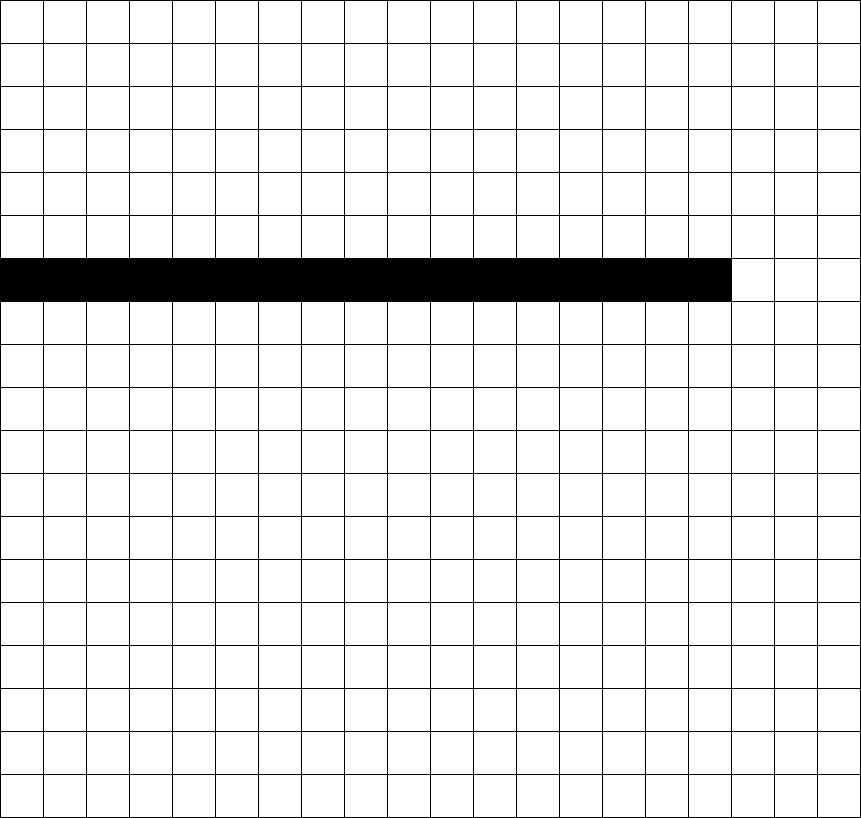
\includegraphics[scale=0.82]{images/m5.png}
    \caption{Hand Crafted Map 2}
    \label{fig: rep_Hand Crafted Map 2}
\end{figure}

\begin{table}[h!] 
\footnotesize
\centering


\begin{tabular}{|cc|c|c|c|c|c|}
\hline
\multicolumn{2}{|c|}{\textbf{Nr.}} & \textbf{Success Rate} & \textbf{Distance} & \textbf{Time} & \textbf{Distance Left}\\
\hline
\hline
\multicolumn{2}{|c|}{\cellcolor{lightgray!20} \hyperref[tab: evalalgorithms]{0}} & 100.0\% (I: 0\%) & 10.24 (A*: 10.24) (I: 0\%) & 0.0055s & 0.0\\
\hline
\hline
\multicolumn{2}{|c|}{\cellcolor{red!40} \hyperref[tab: evalalgorithms]{1}} & 78.0\% (I: -22.0\%) & 7.5 (A*: 7.48) (I: -0.27\%) & 0.02s & 2.04\\
\hline
\multicolumn{2}{|c|}{\cellcolor{red!20} \hyperref[tab: evalalgorithms]{2}} & 80.0\% (I: -20.0\%) & 8.05 (A*: 7.92) (I: -1.64\%) & 0.0206s & 2.01\\
\hline
\multicolumn{2}{|c|}{\cellcolor{red!20} \hyperref[tab: evalalgorithms]{3}} & 98.0\% (I: -2.0\%) & 10.15 (A*: 10.09) (I: -0.59\%) & 0.0255s & 0.16\\
\hline
\multicolumn{2}{|c|}{\cellcolor{red!20} \hyperref[tab: evalalgorithms]{4}} & 78.0\% (I: -22.0\%) & 7.48 (A*: 7.48) (I: 0\%) & 0.0196s & 1.77\\
\hline
\multicolumn{2}{|c|}{\cellcolor{red!20} \hyperref[tab: evalalgorithms]{5}} & 98.0\% (I: -2.0\%) & 10.22 (A*: 10.17) (I: -0.49\%) & 0.0253s & 0.32\\
\hline
\hline
\multicolumn{2}{|c|}{\cellcolor{blue!20} \hyperref[tab: evalalgorithms]{6}} & 78.0\% (I: -22.0\%) & 7.89 (A*: 7.48) (I: -5.48\%) & 0.0429s & 1.77\\
\hline
\multicolumn{2}{|c|}{\cellcolor{blue!40} \hyperref[tab: evalalgorithms]{7}} & 76.0\% (I: -24.0\%) & 7.89 (A*: 7.36) (I: -7.2\%) & 0.0434s & 1.97\\
\hline
\multicolumn{2}{|c|}{\cellcolor{blue!20} \hyperref[tab: evalalgorithms]{8}} & 96.0\% (I: -4.0\%) & 10.16 (A*: 10.13) (I: -0.3\%) & 0.0481s & 0.34\\
\hline
\multicolumn{2}{|c|}{\cellcolor{blue!20} \hyperref[tab: evalalgorithms]{9}} & 76.0\% (I: -24.0\%) & 7.36 (A*: 7.36) (I: 0\%) & 0.0423s & 1.92\\
\hline
\multicolumn{2}{|c|}{\cellcolor{blue!20} \hyperref[tab: evalalgorithms]{10}} & 100.0\% (I: 0\%) & 10.31 (A*: 10.24) (I: -0.68\%) & 0.0485s & 0.0\\
\hline
\hline
\multicolumn{2}{|c|}{\cellcolor{orange!40} \hyperref[tab: evalalgorithms]{11}} & 100.0\% (I: 0\%) & 10.35 (A*: 10.24) (I: -1.07\%) & 0.4895s & 0.0\\
\hline
\multicolumn{1}{|M{0.15cm}}{\cellcolor{cyan!40}} & \multicolumn{1}{M{0.15cm}|}{\cellcolor{blue!40} \hspace*{-0.5cm}\hyperref[tab: evalalgorithms]{12}} & 100.0\% (I: 0\%) & 10.43 (A*: 10.24) (I: -1.86\%) & 0.1472s & 0.0\\
\hline
\multicolumn{1}{|M{0.15cm}}{\cellcolor{cyan!40}} & \multicolumn{1}{M{0.15cm}|}{\cellcolor{red!40} \hspace*{-0.5cm}\hyperref[tab: evalalgorithms]{13}} & 100.0\% (I: 0\%) & 10.87 (A*: 10.24) (I: -6.15\%) & 0.0548s & 0.0\\
\hline
\multicolumn{1}{|M{0.15cm}}{\cellcolor{cyan!40}} & \multicolumn{1}{M{0.15cm}|}{\cellcolor{orange!40} \hspace*{-0.5cm}\hyperref[tab: evalalgorithms]{14}} & 100.0\% (I: 0\%) & 10.24 (A*: 10.24) (I: 0\%) & 0.5487s & 0.0\\
\hline
\end{tabular}


\bigskip

\begin{tabular}{|cc|c|c|}
\hline
\multicolumn{2}{|c|}{\textbf{Nr.}} & \textbf{Pick Ratio}\\
\hline
\hline
\multicolumn{2}{|c|}{\cellcolor{orange!40} \hyperref[tab: evalalgorithms]{11}} & [72.0, 6.0, 20.0, 2.0, 0.0, 0.0, 0.0, 0.0, 0.0, 0.0]\%\\
\hline
\hline
\multicolumn{1}{|M{0.15cm}}{\cellcolor{cyan!40}} & \multicolumn{1}{M{0.15cm}|}{\cellcolor{orange!40} \hspace*{-0.5cm}\hyperref[tab: evalalgorithms]{14}} & [74.0, 8.0, 16.0, 2.0, 0.0, 0.0, 0.0, 0.0, 0.0, 0.0]\%\\
\hline
\end{tabular}


\bigskip

\begin{tabular}{|cc|c|c|c|c|M{3cm}|}
\hline
\multicolumn{2}{|c|}{\textbf{Nr.}} & \textbf{GK Improvement} & \textbf{GK Distance} & \textbf{GK Distance Left} & \textbf{WP} & \textbf{WP In-Between Distance}\\
\hline
\hline
\multicolumn{1}{|M{0.15cm}}{\cellcolor{cyan!40}} & \multicolumn{1}{M{0.15cm}|}{\cellcolor{blue!40} \hspace*{-0.5cm}\hyperref[tab: evalalgorithms]{12}} & 87.29\% & 8.0 & 1.97 & 3.02 & 5.64\\
\hline
\multicolumn{1}{|M{0.15cm}}{\cellcolor{cyan!40}} & \multicolumn{1}{M{0.15cm}|}{\cellcolor{red!40} \hspace*{-0.5cm}\hyperref[tab: evalalgorithms]{13}} & 100.0\% & 10.87 & 0.0 & 2.1 & 8.03\\
\hline
\multicolumn{1}{|M{0.15cm}}{\cellcolor{cyan!40}} & \multicolumn{1}{M{0.15cm}|}{\cellcolor{orange!40} \hspace*{-0.5cm}\hyperref[tab: evalalgorithms]{14}} & 100.0\% & 10.24 & 0.0 & 2.06 & 8.12\\
\hline
\end{tabular}


\bigskip

\begin{tabular}{|cc|c|c|c|c|c|}
\hline
\multicolumn{2}{|c|}{\textbf{Nr.}} & \textbf{Total Search} & \textbf{Total Fringe} & \textbf{Session Search} & \textbf{Session Fringe}\\
\hline
\hline
\multicolumn{2}{|c|}{\cellcolor{lightgray!20} \hyperref[tab: evalalgorithms]{0}} & 16.25\% & 8.17\% & 16.25\% & 8.17\%\\
\hline
\hline
\multicolumn{1}{|M{0.15cm}}{\cellcolor{cyan!40}} & \multicolumn{1}{M{0.15cm}|}{\cellcolor{blue!40} \hspace*{-0.5cm}\hyperref[tab: evalalgorithms]{12}} & 13.32\% (I: 18.03\%) & 7.85\% (I: 3.92\%) & 5.13\% (I: 68.43\%) & 3.22\% (I: 60.59\%)\\
\hline
\multicolumn{1}{|M{0.15cm}}{\cellcolor{cyan!40}} & \multicolumn{1}{M{0.15cm}|}{\cellcolor{red!40} \hspace*{-0.5cm}\hyperref[tab: evalalgorithms]{13}} & 15.88\% (I: 2.28\%) & 7.59\% (I: 7.1\%) & 7.93\% (I: 51.2\%) & 4.13\% (I: 49.45\%)\\
\hline
\multicolumn{1}{|M{0.15cm}}{\cellcolor{cyan!40}} & \multicolumn{1}{M{0.15cm}|}{\cellcolor{orange!40} \hspace*{-0.5cm}\hyperref[tab: evalalgorithms]{14}} & 14.94\% (I: 8.06\%) & 7.49\% (I: 8.32\%) & 7.71\% (I: 52.55\%) & 4.16\% (I: 49.08\%)\\
\hline
\end{tabular}


\caption{\textbf{Analyser} complex analysis on the hand crafted map described in Figure \ref{fig: rep_Hand Crafted Map 2} with 50 random agent/goal positions}
\label{tab: eval_complex_analysis_map_5} 
\end{table}

\begin{itemize}
    \item The performance of all algorithms is greatly boosted as the hand crafted map is quite simple in layout, but was used to test the ability of the algorithm to go around long walls which was an issue in paper \cite{nicola2018lstm}
    \item Algorithm \hyperref[tab: evalalgorithms]{14} - has 100\% GK Improvement and 0\% distance improvement rate, which matches the A* performance exactly
\end{itemize}

\pagebreak